\chapter{The \acs{LHC} and the \acs{CMS} experiment}
\label{chap:CMSLHC}

\section{The \acs{LHC}}
\label{sec:CMSLHC_LHC}

The \acf{LHC} \cite{lhc-machine}  is a $26.7\,\kilo\metre$ long synchrotron hadron accelerator and collider below the surface of the 
Franco-Swiss border near Geneva. It
is installed in the tunnel that previously hosted the \acf{LEP} accelerator \cite{lep-design}
that was operated by \acf{CERN} between 1989 and 2000.

The \ac{LHC} was designed to collide two beams of protons %with each other 
at centre-of-mass
energies ($\sqrt{s}$) of up to $14\,\TeV$. It therefore consists of two rings in which the beams
of protons are individually accelerated. In addition to colliding beams of protons, the \ac{LHC}
is also used for proton-lead and lead-lead collisions.
\begin{figure}[h!]
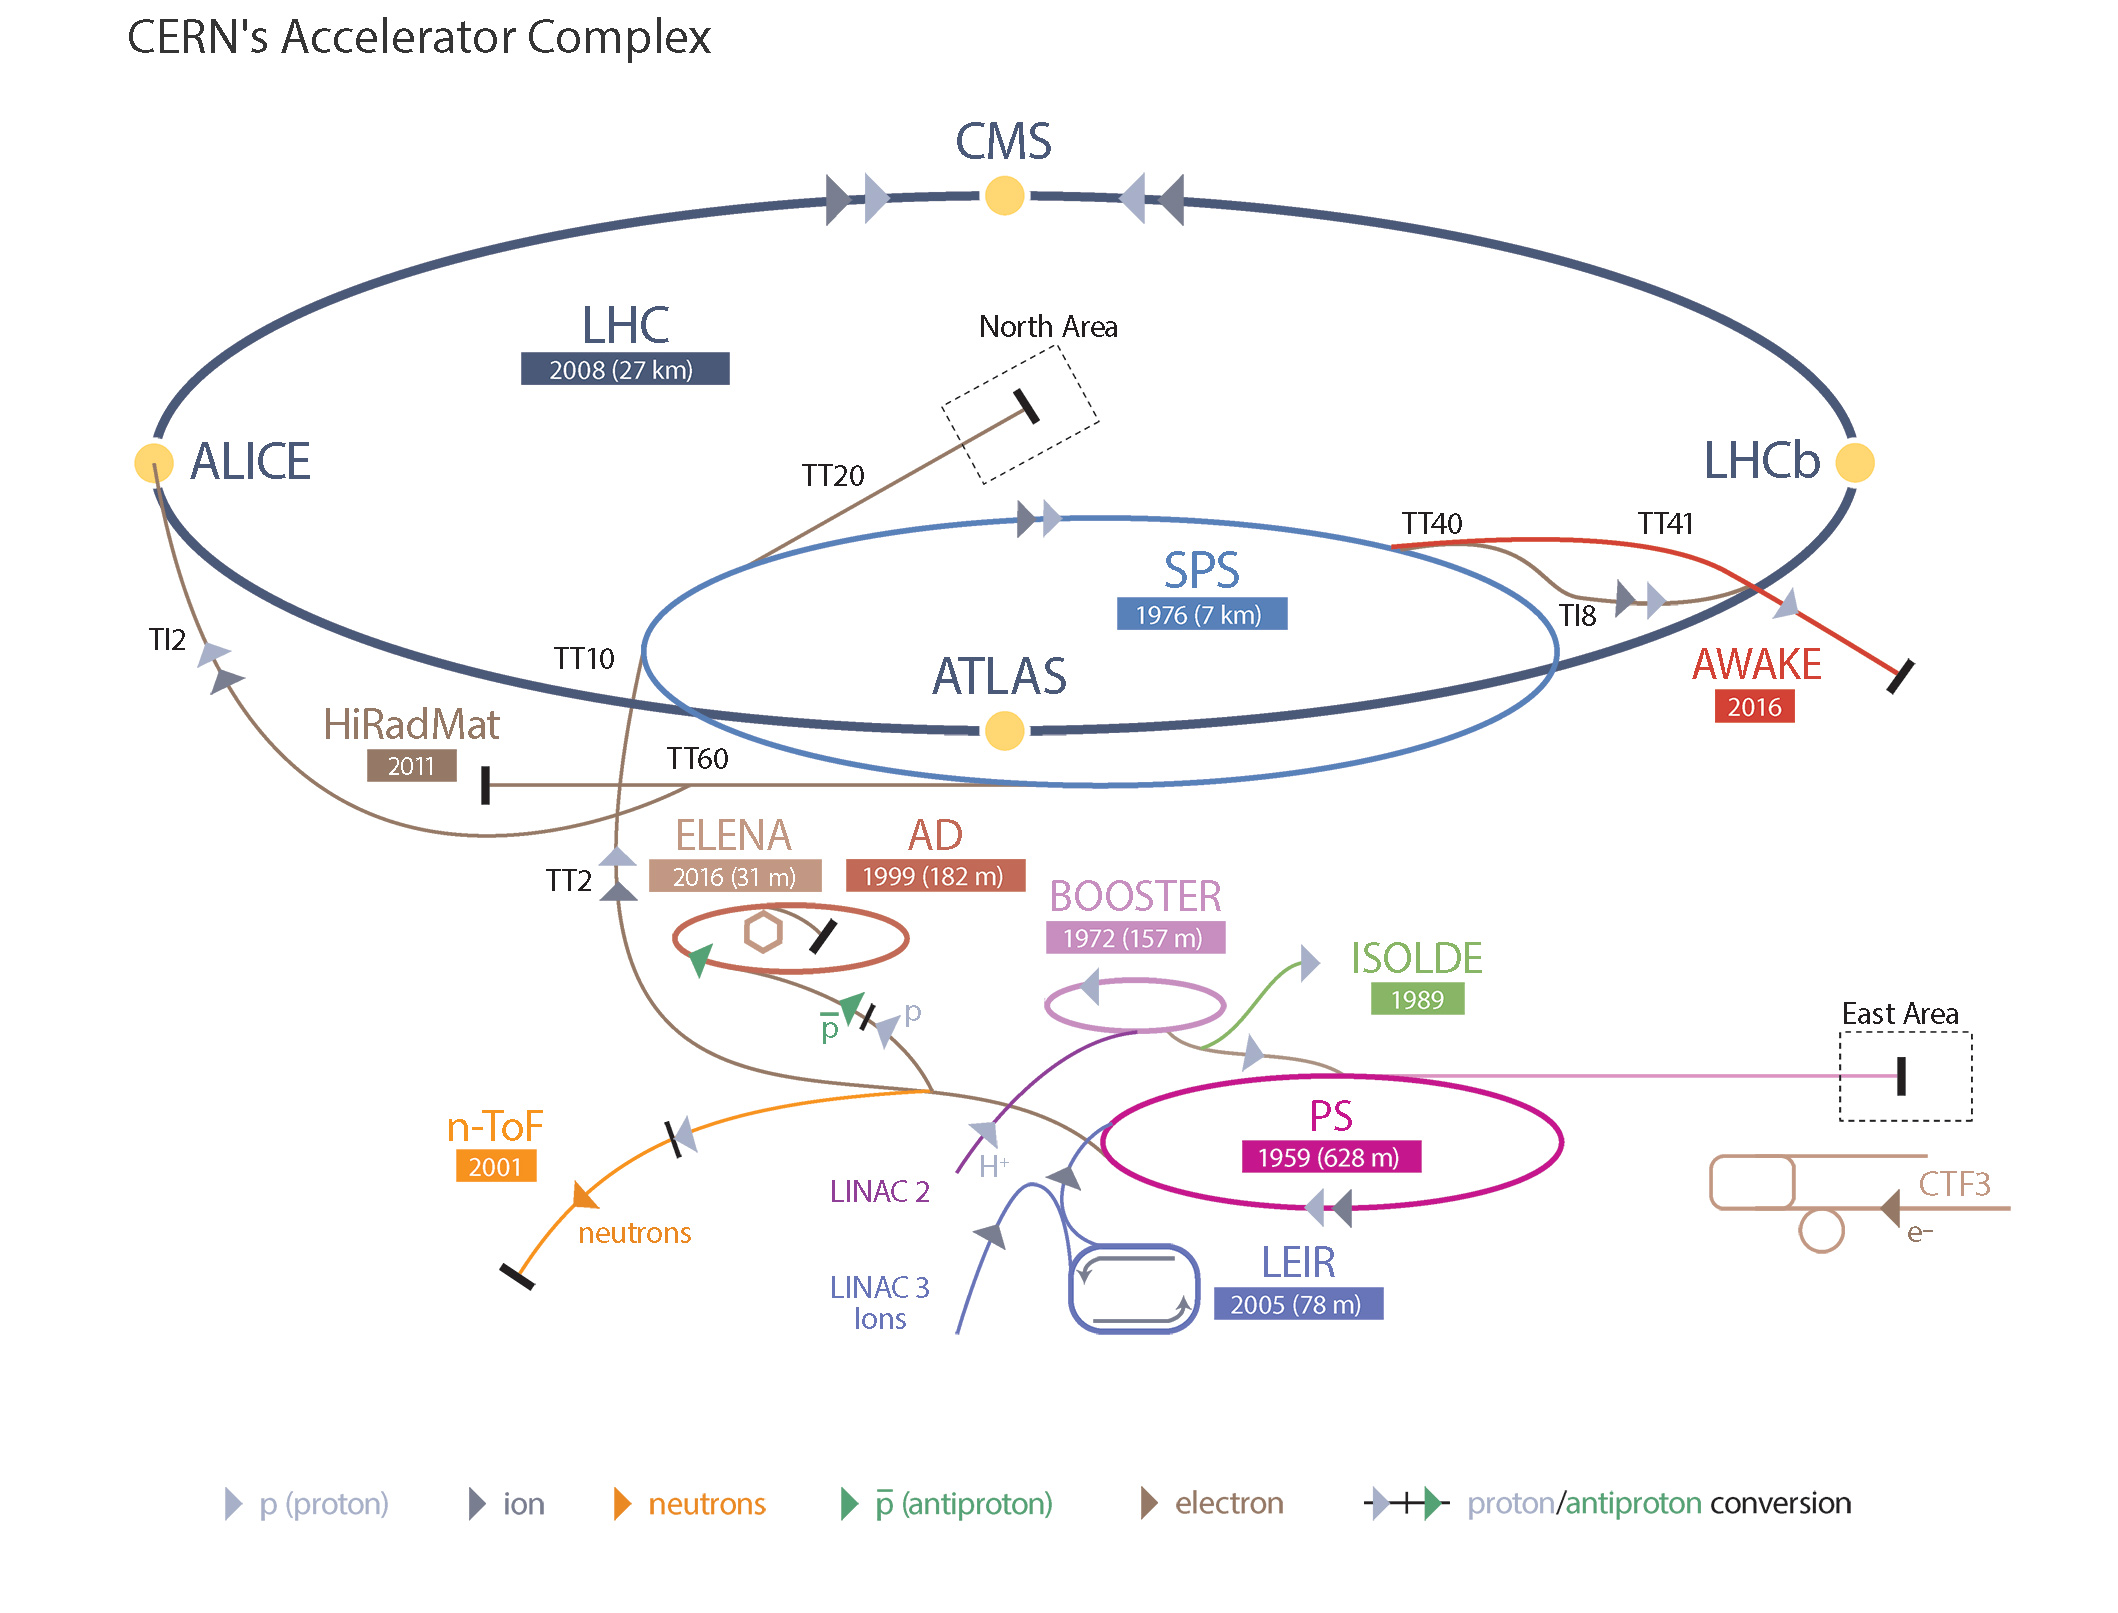
\includegraphics[width=\textwidth]{./Detector/Plots/LHC_default.jpg}
\caption[Schematic of the CERN accelerator complex.]{Schematic of the \ac{CERN} accelerator complex \cite{lhc-schematic}.}
\label{fig:lhc_schematic}
\end{figure}

The \ac{LHC} does not operate on its own: the protons are fed into
it via a chain of accelerators. Figure \ref{fig:lhc_schematic} shows a schematic
of the \ac{CERN} accelerator complex.
Protons originate from hydrogen gas, where electrons are stripped off the 
hydrogen atoms using an electric field. The protons then pass through an injector
chain which increases the energy of the protons in several steps. After the protons
are created from the hydrogen gas they are accelerated to an energy of
$50\,\MeV$ in the Linac~2 linear accelerator. They are then passed on to the
\acf{PSB} which accelerates the protons until they reach an energy of $1.4\,\GeV$.
The next accelerator in the chain, the \acf{PS}, further accelerates the protons to $25\,\GeV$,
with the \acf{SPS} bringing the energy up to $450\,\GeV$. When this energy has been 
reached the protons are injected into the \ac{LHC} in two counter-rotating
beams. In the \ac{LHC} ring the beams are further accelerated to the required centre-of-mass energy
by eight \ac{RF} cavities. At design operation the beams consist of 2808 proton bunches each made up 
of $\mathcal{O}(10^{11})$ protons, spaced $25\,\ns$ apart. The beams are kept in circulation
using 1232 niobium-titanium superconducting dipole magnets, cooled to operate at 
a temperature of $1.9\,\kelvin$ and generating magnetic fields of up to $8.4\,\tesla$.
The beams collide at four points
around the \ac{LHC} ring, where the collisions are recorded by the ATLAS\cite{atlas-jinst}, 
\acs{CMS}\cite{cms-jinst}, ALICE\cite{alice-jinst}, and LHCb\cite{lhcb-jinst} detectors.

The processes the \ac{LHC} was built to study have a small cross section
compared with the total proton-proton (p-p) inelastic cross section, as seen from figure
\ref{fig:stirling_xs}. For example, the production cross section of the
\ac{SM} Higgs boson is 9--10 orders of magnitude smaller than the total p-p cross section.
In order to be able to study these relatively rare processes  
the \ac{LHC} operates at high instantaneous luminosity, defined as
\begin{equation}\label{eqn:CMSLHC_luminosity}
\mathcal{L} = \frac{N_b^2n_bf_{\text{rev}}\gamma}{4\pi\epsilon_n\beta^{*}}F,
\end{equation}
where $N_b$ is the number of protons per bunch, $n_b$ the number of
bunches per beam, $f_{\text{rev}}$ the revolution frequency, $\gamma$ the 
Lorentz factor, $\epsilon_n$ the normalised beam
emittance, $\beta^{*}$ the $\beta$-function at the interaction point and F a reduction
factor due to the crossing angle. 

\begin{figure}[h!]
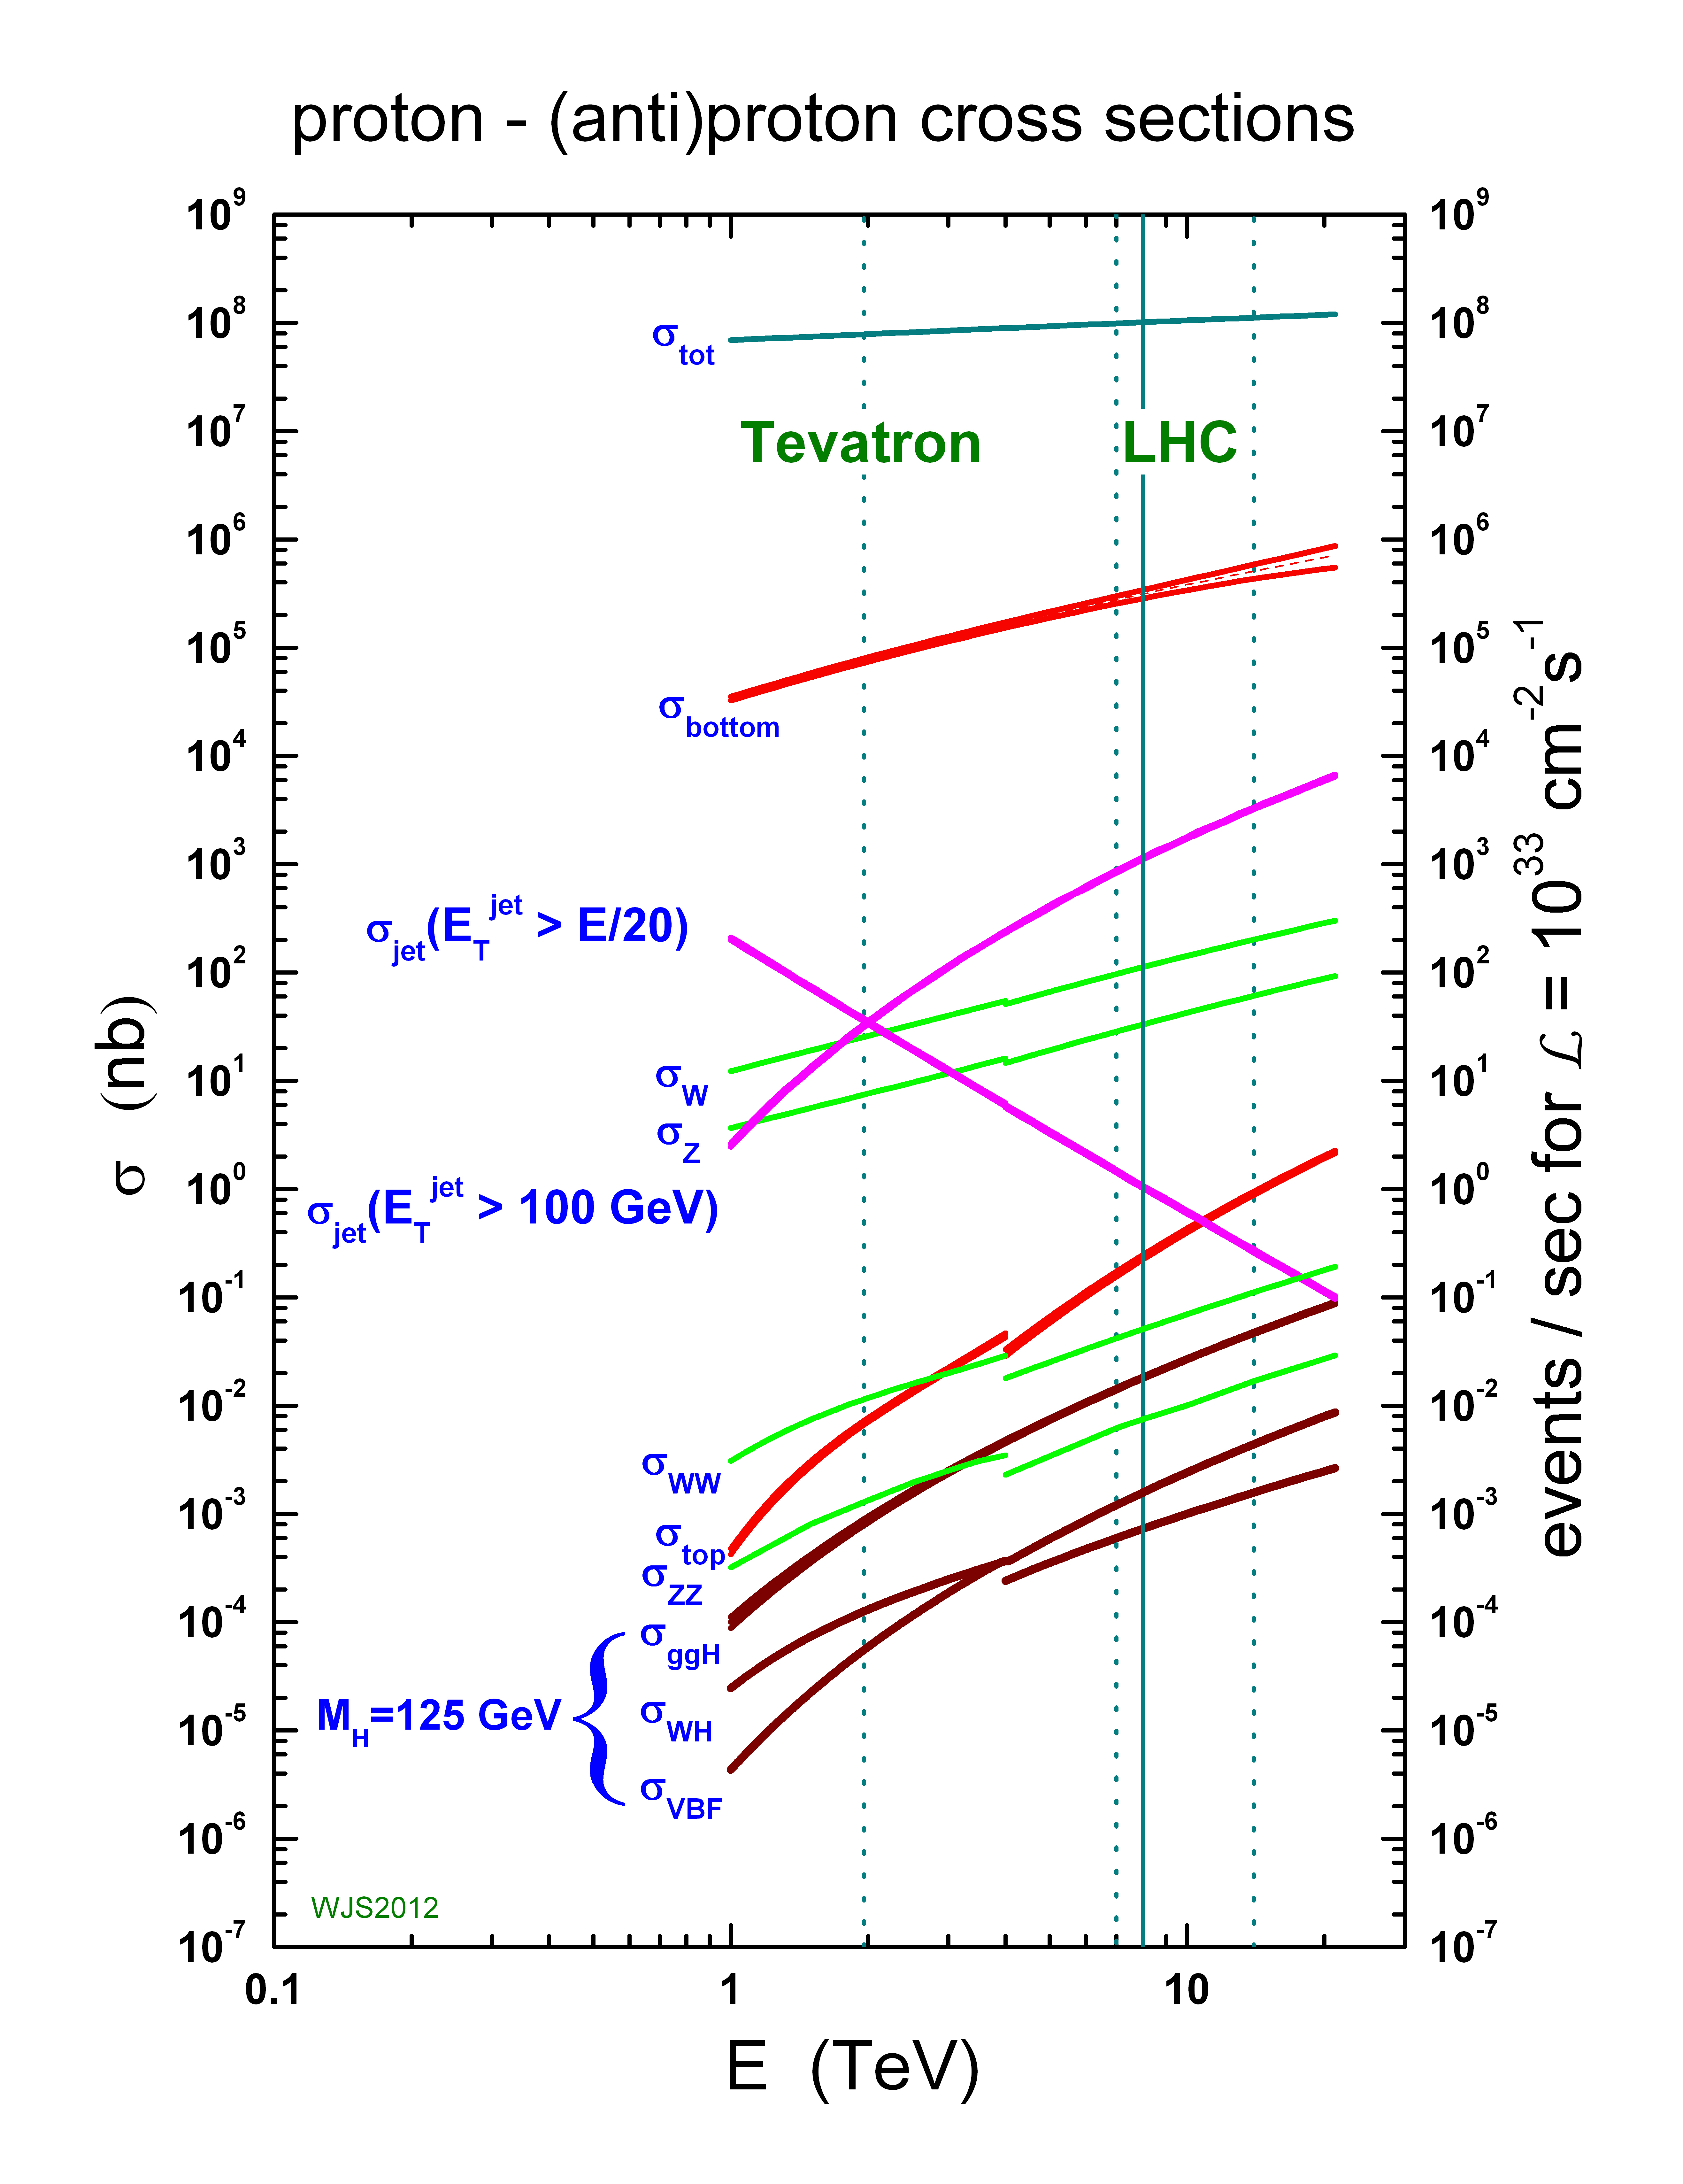
\includegraphics[width=0.5\textwidth]{./Detector/Plots/crosssections2013.jpg}
\caption[Total p-p cross section, and the cross sections for
several processes studied at the LHC.]{Total p-p cross section, $\sigma^{\text{tot}}$, and the cross sections
for several processes studied at the LHC as a function of $\sqrt{s}$ \cite{stirling-crosssection}.
The cross sections of these processes
are often many orders of magnitude smaller than the total p-p cross section.}
\label{fig:stirling_xs}
\end{figure}

The \ac{LHC} began its first physics run in May 2010, colliding protons at
$\sqrt{s}=7\,\TeV$, and continued operation until the end of 2012. This period is known
collectively as \ac{LHC} Run 1. After this the 
two-year \ac{LS1} was used to upgrade the \ac{LHC} and the detectors for collisions at a
$\sqrt{s}$ of $13\text{--}14\,\TeV$. In April 2015 the \ac{LHC} restarted with collisions at 
$\sqrt{s}=13\,\TeV$, marking the start of Run 2. The integrated luminosity delivered to the \ac{CMS} experiment, separated by running year, is shown in
figure \ref{fig:CMSLHC_intlumi}.

\begin{figure}[h!]
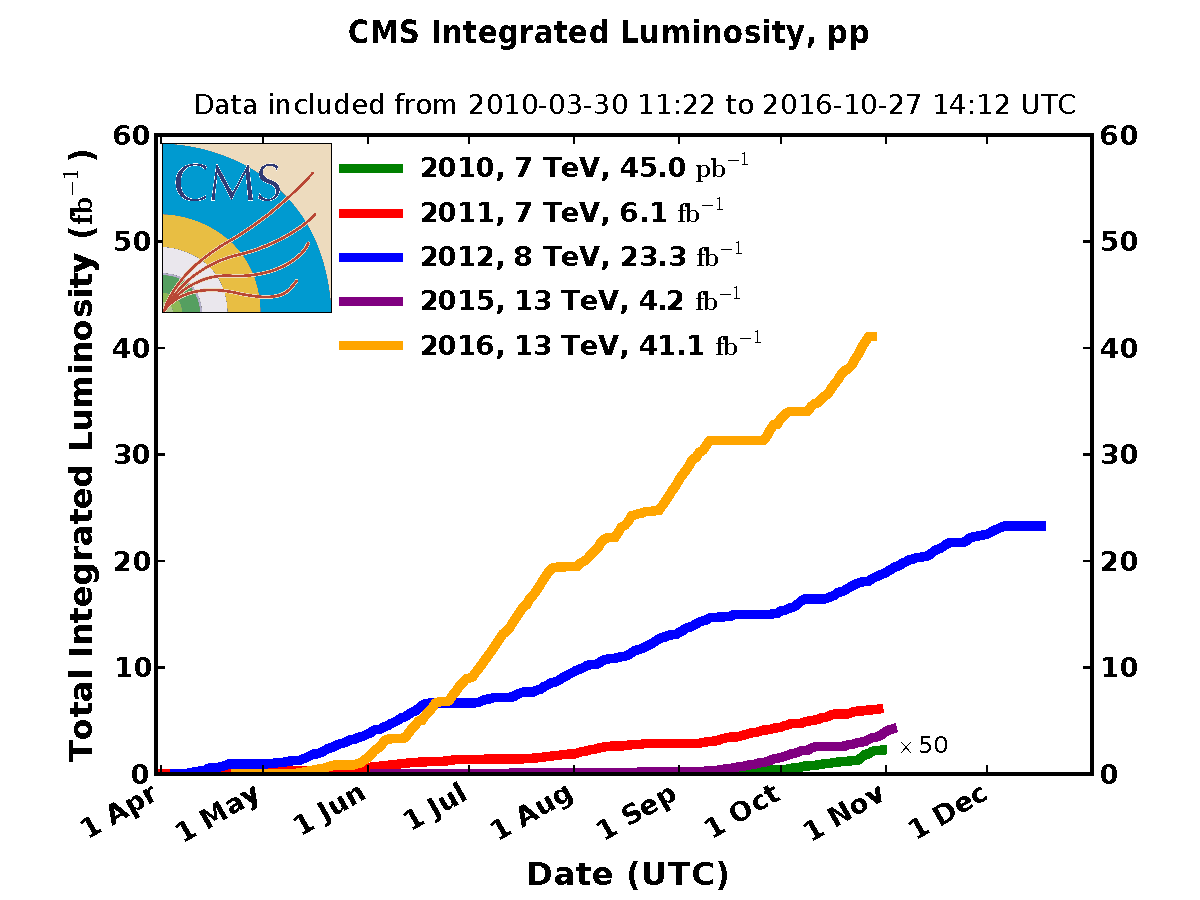
\includegraphics[width=0.85\textwidth]{./Detector/Plots/int_lumi_cumulative_pp_2.pdf}
\caption[Cumulative integrated luminosity delivered to CMS
for p-p collisions at the LHC, separated by running year.]{Cumulative integrated luminosity delivered to \ac{CMS} for p-p collisions at the \ac{LHC}, separated
by running year \cite{cms-lumi-public}.}
\label{fig:CMSLHC_intlumi}
\end{figure}

The data-taking efficiency of CMS is not 100\%, as parts of the detector might be
switched off while collisions are ongoing. In 2012 the data-taking 
efficiency was 93.5\%, in 2015 it was 90.3\% and in 2016 it was 92.0\%.
Only a subset of the recorded data is used for analysis.
Data are
certified as good for use in analyses if it is known that all relevant sub-detectors
were functioning correctly. In 2012 the certification efficiency was 90.4\%, 
meaning all sub-detectors were working well for a dataset corresponding to $19.7\,\invfb$. %MAYBE COME BACK TO LATER?
Due to cryogenic issues the certification efficiency with the magnet operating
at $3.8\,\tesla$ was 60.4\% in 2015, leading to $2.3\,\invfb$ of 
analysable data for which the full detector was operational. An additional $0.6\,\invfb$
was taken with the \ac{CMS} magnet switched off. For the full 2016 p-p running period
the certification efficiency was 95.0\%, resulting in $35.9\,\invfb$ of data marked good %FIXME: certification efficiency
for use in analyses.

The \ac{LHC} was designed for p-p collisions with a nominal
peak luminosity of $10^{34}\,\lumiunits$. In 2012 peak
luminosities of $7.7\times 10^{33}\,\lumiunits$ were reached, with the peak luminosity in
2015 being $5.1\times 10^{33}\,\lumiunits$. Since July 2016
the \ac{LHC} has been operating at instantaneous luminosities upwards of the 
design luminosity, with peak luminosities of $1.5\times10^{34}\,\lumiunits$ reached
in October 2016 \cite{cms-lumi-public}.

Multiple p-p collisions per bunch crossing are likely to occur due to the high
operating luminosity. 
Additional interactions on top of events of 
interest are referred to as pileup. The average number of interactions %FIXME: make clear that they are unintersting?
per bunch crossing was 21 in 2012\cite{cms-lumi-public}. The average number of
interactions per bunch crossing was lower than this at the start of Run 2, with
an average of 14 interactions per bunch crossing for the data collected
during 2015 \cite{CMS-PAS-HIG-16-006}. In the data-taking period up to August 2016 the average number of interactions
per bunch crossing increased to 24 \cite{CMS-PAS-HIG-16-037}.

\section{The \acs{CMS} detector}
\label{sec:CMSLHC_CMS}
To meet the demands of the \ac{LHC} physics programme, the
 \ac{CMS} detector was designed to have a high sensitivity in searches 
for new physics at the $\TeV$ scale and to be able to 
function in the challenging high-luminosity environment.
The detector is $21.6\,\metre$ long, $14.6\,\metre$ in diameter, and weighs
$12\,500$ tonnes \cite{cms-jinst}. It consists of several sub-detectors, arranged parallel
to the beam axis in the barrel region and perpendicular to it in the endcaps, as illustrated
in figure \ref{fig:cms_detector}.
\begin{figure}[h!]
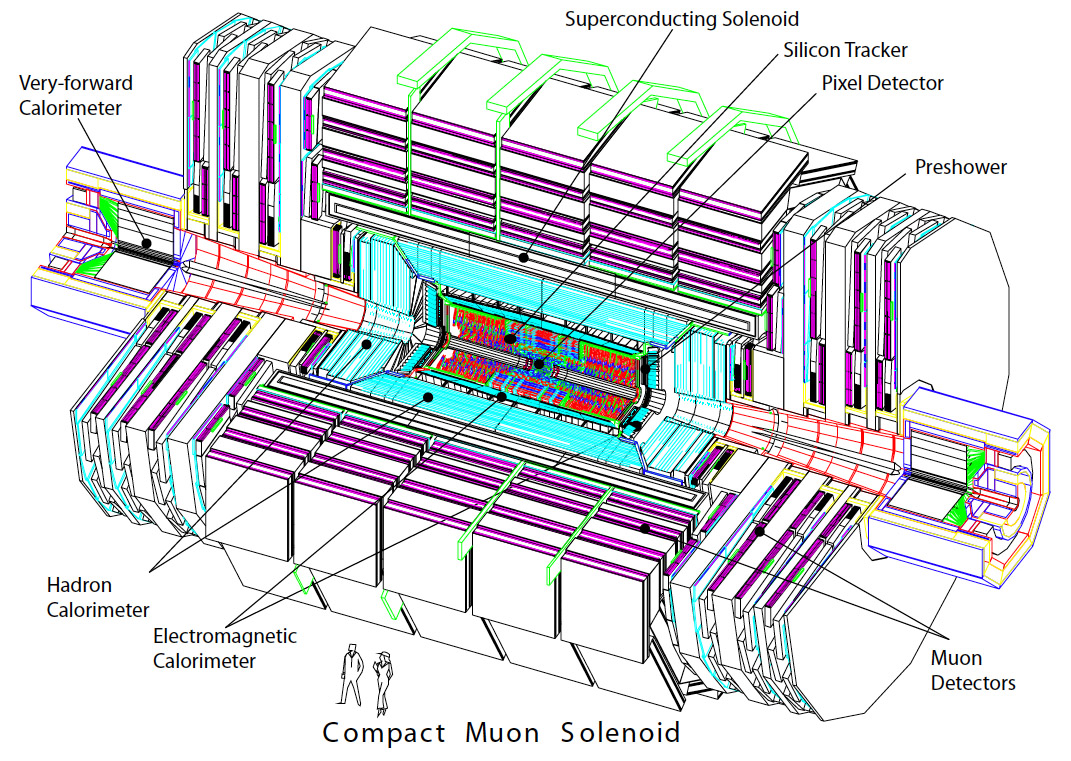
\includegraphics[width=0.8\textwidth]{./Detector/Plots/cms.png}
\caption[A cutaway view of the CMS detector, indicating the different sub-components of the detector.]{A cutaway view of the \ac{CMS} detector \cite{cms-jinst}, indicating the
different sub-components of the detector.}
\label{fig:cms_detector}
\end{figure}

The silicon tracker, a cylinder $5.8\,\metre$ in length and $2.6\,\metre$ in
diameter, surrounds the interaction point. The tracker is 
surrounded by the lead-tungstate \ac{ECAL}, which is enclosed
by the brass scintillator \ac{HCAL}.
The tracking and calorimeter systems are surrounded by a superconducting
solenoid, $13\,\metre$ long, $6\,\metre$ in diameter and operating at $3.8\,\tesla$.
Charged particles are bent in this magnetic field, allowing for precise 
measurement of their momentum. Gaseous muon detectors are embedded in the 
iron return yoke of the solenoid.

For the measurement of physical quantities \ac{CMS} uses a coordinate
system with the origin centred at the nominal collision point
inside the experiment. The $y$ axis points vertically upward, the $x$ axis
points radially inward toward the centre of the \ac{LHC} ring. The \mbox{$z$ axis}
points along the beam direction. As such the transverse momentum and energy, 
\pT~and \ET, are defined by the $x$- and $y$-components of the momentum and energy.
The azimuthal angle $\phi$ is measured in the $x$-$y$ plane with respect to the $x$ axis  
and the polar angle $\theta$ is measured with respect to the $z$ axis. A coordinate
more frequently used than the polar angle is the pseudorapidity $\eta = -\ln{[\tan{\frac{\theta}{2}}]}$. %Look up: differences in eta are lorentz-invariant
Distances in the $\eta$-$\phi$ plane are given as $\Delta R = \sqrt{(\Delta\eta)^2+(\Delta\phi)^2}$. 

The subsystems of the \ac{CMS} detector will be described in more detail in the 
next sections.

\subsection{Tracker}
\label{sec:CMSLHC_CMS_tracker}
The tracker \cite{cms-jinst} is the sub-detector closest to the interaction point. It
is used for accurate reconstruction of charged particle trajectories and 
the precise reconstruction of primary (collision) and secondary vertices, the latter being important for
the identification of the in-flight decays of heavy-flavour particles. This means a small impact parameter
resolution needs to be achieved, for which a highly granular system is required. 
Due to the large number of particles emerging from 
each collision, on average 1000 per bunch crossing at design operation, the 
system also needs to be able to respond quickly in order to reconstruct trajectories accurately.
At the same time, this large particle flux calls for a 
radiation-hard design that is able to survive in this harsh environment
for a long period of time. These requirements motivate the use of a silicon tracking
system. 

In a silicon tracking system the positions of particles are recorded
via the creation of drifting electron-hole pairs.
When a charged particle passes through the silicon an electron-hole pair
is created, which drift under an applied electric field and produce a current
that can be read out. %LEARN A BIT MORE ABOUT THIS

The tracker, providing coverage up to $|\eta|<2.5$, consists of 
several different components. A schematic of the tracking detector, indicating
the locations of these components, is given in figure \ref{fig:CMS_tracker}.
The pixel detector is the closest to the interaction point.
It is composed
of 66 million silicon pixels, each $100\,\micron\,\times\,150\,\micron$ in size.
The choice of this pixel size is driven by the desired spatial resolution,
which is $15$--$20\,\micron$ in the $r$-$\phi$ and $z$~directions. Such a
precise resolution allows for 3D vertex reconstruction. The pixel
detector consists of three layers of pixels in the barrel region, with two pixel disks 
placed in the endcap region at either side. The barrel layers sit at radii of
$4.4$, $7.3$ and $10.2\,\cm$ and extend out to $z=\pm\,26.5\,\cm$. The disks are placed
at $z=\pm\,34.5\,\cm$ and $z=\pm\,46.5\cm$. With this layout the pixel tracker can
provide three precise position measurements along each charged particle trajectory.

\begin{figure}[h!]
\begin{center}
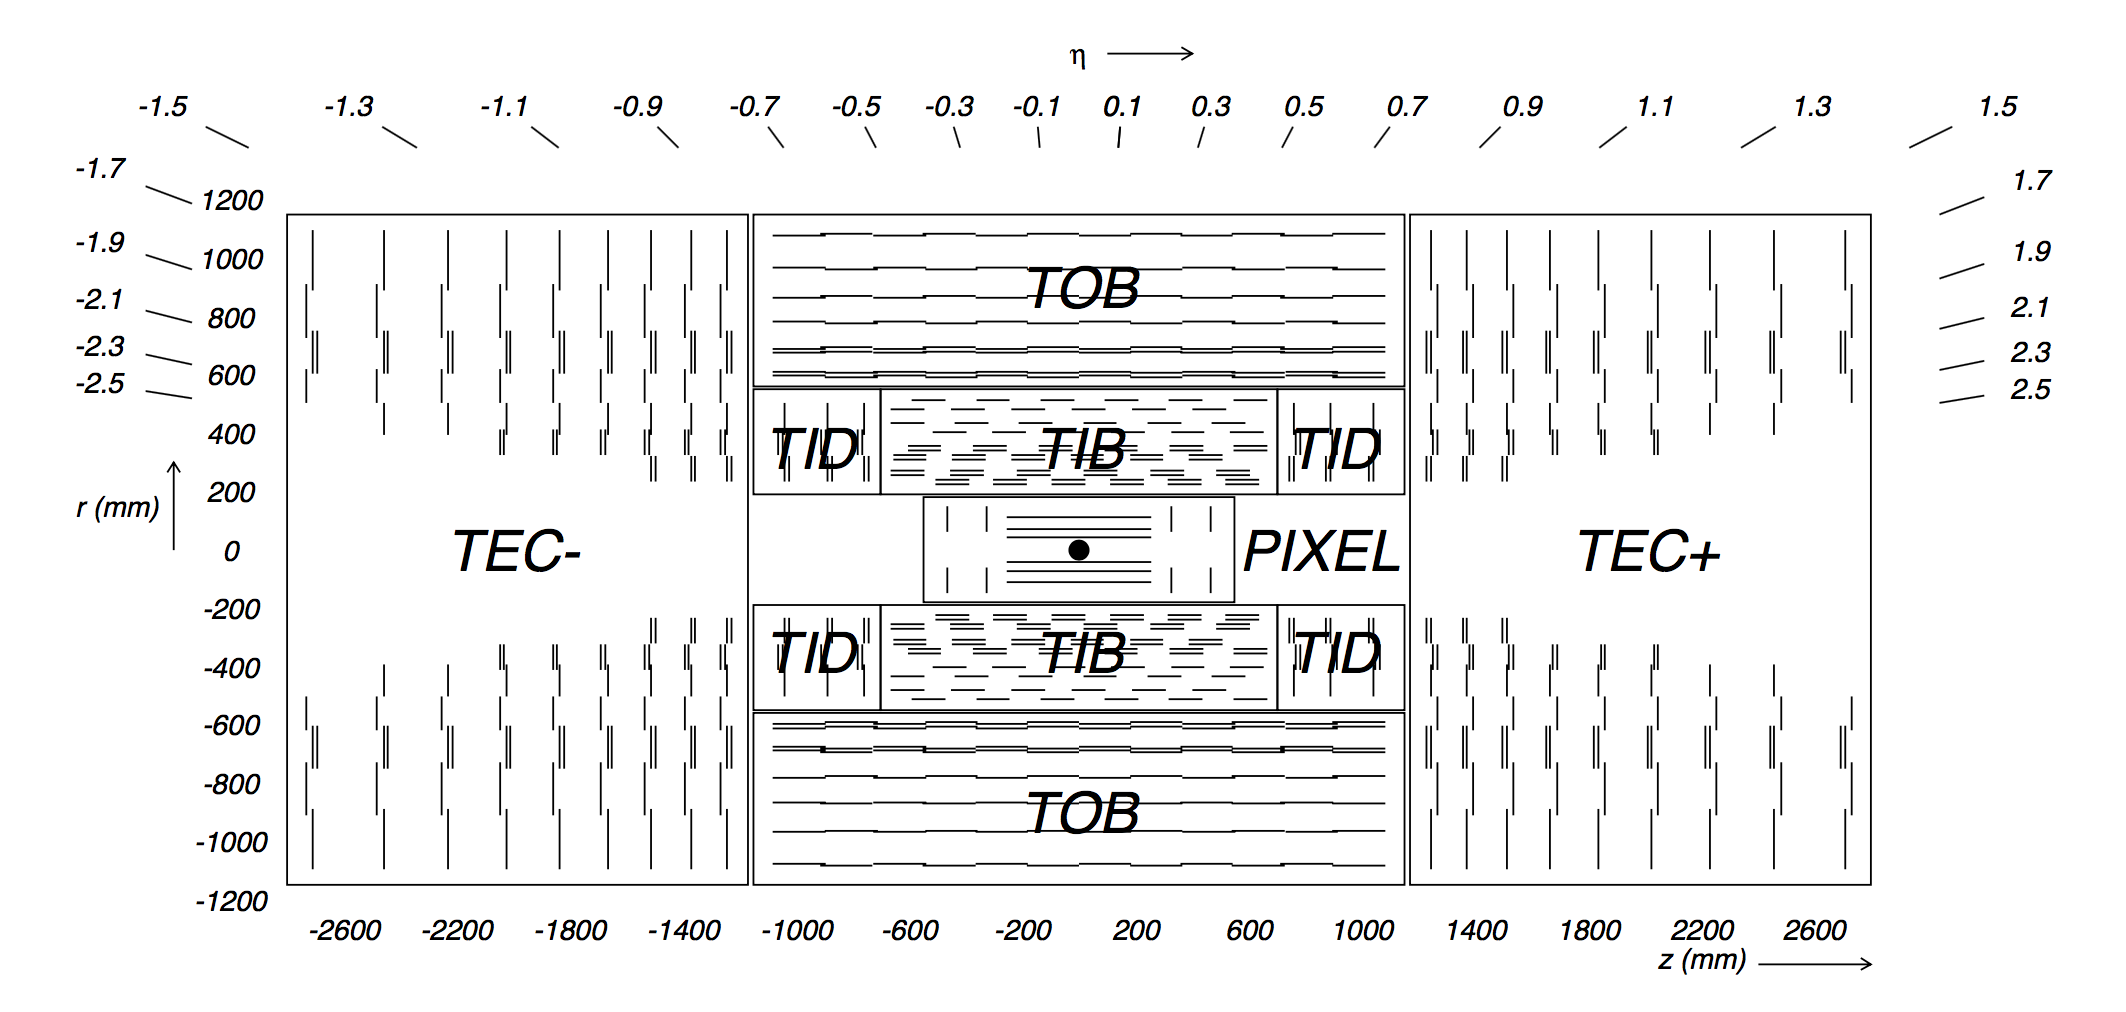
\includegraphics[width=0.9\textwidth]{./Detector/Plots/Tracker.png}
\caption[Schematic of the CMS tracker in the 
$r$-$z$ plane, indicating the positions of the pixel and
strip detectors.]{Schematic of the CMS tracker in the $r$-$z$ plane, indicating the
positions of the pixel and strip detectors \cite{cms-jinst}. Each line 
on the figure represents a detector module.}
\label{fig:CMS_tracker}
\end{center}
\end{figure}

Around the pixel detector the tracking system is made up of a silicon
strip detector divided into four sub-systems. The first part of the
silicon strip tracker consists of the \ac{TIB} and \ac{TID}, providing four layers of
silicon strip detectors in the barrel plus three disks at both ends. These two systems
extend out up to a radius of $55\,\cm$. The barrel layers and disks each consist
of silicon strips which are $10\,\cm$ long, $80$--$141\,\micron$ wide and $320\,\micron$ thick. The \ac{TIB} and \ac{TID}
provide four measurements of the $r$-$\phi$ position with a resolution of $23$--$35\,\micron$. 
The \ac{TIB} and \ac{TID} are surrounded by the \ac{TOB}, which consists of six layers of silicon strip sensors extending
up to an outer radius of $116\,\cm$ and up to $z=\pm\,118\,\cm$. The strips in the \ac{TOB} are $500\,\micron$ thick, 
around $25\,\cm$ long and $122$--$183\,\micron$ 
wide providing six measurements of $r$ and $\phi$, with a resolution
of $35$--$53\,\micron$. Beyond the $z$ range covered by the \ac{TOB}, coverage is provided by the \ac{TEC},
consisting of nine disks of strips. In the \ac{TEC} the strip thickness ranges from $320$--$500\,\micron$ and 
the the strip width ranges from $97$--$184\,\micron$. %FIXME: look up why
This part of the system provides up to nine $\phi$ measurements.

Some of the strip modules in the detector carry a second strip detector module mounted back-to-back with a stereo angle %FIXME WTF?
of $100\,$mrad, in order to provide measurements of the \mbox{$z$ coordinate} in the barrel. This is achieved with a resolution of $230$--$530\,\micron$.

The pixel tracker was upgraded during the extended year-end technical stop in late 2016-early 2017. This upgrade was needed to
maintain the performance of the tracker as the pileup increases throughout the remainder of Run 2 \cite{cms-pixel-upgrade}. %or just replaced?

\subsection{Electromagnetic calorimeter}
\label{sec:CMSLHC_CMS_ecal}
The \ac{ECAL} \cite{cms-jinst} is a hermetic homogeneous calorimeter
made of nearly $76\,000$ lead tungstate (PbWO$_4$) crystals. It has very
good energy resolution, is highly granular and has a fast response, all qualities 
which are needed to be able to detect $\PHiggs\rightarrow \Pphoton\Pphoton$ decays.

The choice of lead tungstate crystals is motivated by the
radiation-hardness of the material in combination with its
short radiation length, small Moli\`ere radius and short scintillation
decay time. With a radiation length of $0.89\,\cm$ and a Moli\`ere radius of $2.2\,\cm$,
lead tungstate crystals allow for the construction of a compact, highly 
granular \ac{ECAL}. The \ac{ECAL} is required to be compact 
for it to fit inside the bore of the magnet. 
The lead tungstate crystals satisfy the requirements imposed by the \ac{LHC} 
operating parameters as 80\% of the light from the crystals is emitted within $25\,\ns$,
which is the time between two bunch crossings at design operation.
%Moliere radius: characteristic constant of a material giving scale of transverse dimenstion
%of fully contained EM showers. It is the radius of a cylinder containing on average 
%90pct of the shower's energy deposition. Related to radiation length as 
%molrad approx 0.0265X0 (Z+1.2) with Z the atomic number.
%Radiation length: mean distance over which a high energy electron
%loses all but 1/e of its energy by bremmstrahlung and 7/9 of th emean free path for pair production by 
%a high energy photon.

When a high energy electron or photon enters a crystal it starts a
shower producing a cascade of lower energy particles. Electrons lose
energy through bremsstrahlung, with photons undergoing $\Pe^+ \Pe^-$ 
pair production. The shower continues until the photon energy drops below the 
$\Pe^+\Pe^-$ pair production threshold, and ionisation 
starts to dominate for electrons. The shower excites the atoms in the lead-tungstate
crystals, which then emit scintillation light that is converted to a current by the 
photodetectors. To record the light of the crystals amplifying photodetectors need
to be used, with avalanche photodiodes used in the barrel region, and vacuum phototriodes employed
in the endcaps. %Because of the larger radiation levels in the endcaps
As the crystals are 25.8 radiation lengths long, most of the shower
is contained inside them.

Figure \ref{fig:CMS_ECAL} shows a schematic of the \ac{ECAL}, indicating
the sub-systems it is made up of. The \ac{EB} 
covers the pseudorapidity range up to $|\eta|<1.479$, with
crystals of $0.0174 \times 0.0174$ in $\eta$-$\phi$. The \acp{EE}
provide coverage beyond the range of the \ac{EB}, up to $|\eta|<3.0$.
Each endcap is divided into two halves. The preshower detectors, 
which are sampling calorimeters placed in front of the endcaps, cover a range of $1.653<|\eta|<2.6$.
The main use of the preshower detectors is to identify neutral pions decaying to two photons in the 
endcaps. Additionally,
they aid in the identification of electrons and improve the resolution
of the position determination. Each of the two preshower detectors consists
of two layers of lead radiators to initiate the shower, with silicon sensors
placed after each layer of radiators to measure the deposited energy. The 
total thickness of the preshower is three radiation lengths.

\begin{figure}[h!]
\begin{center}
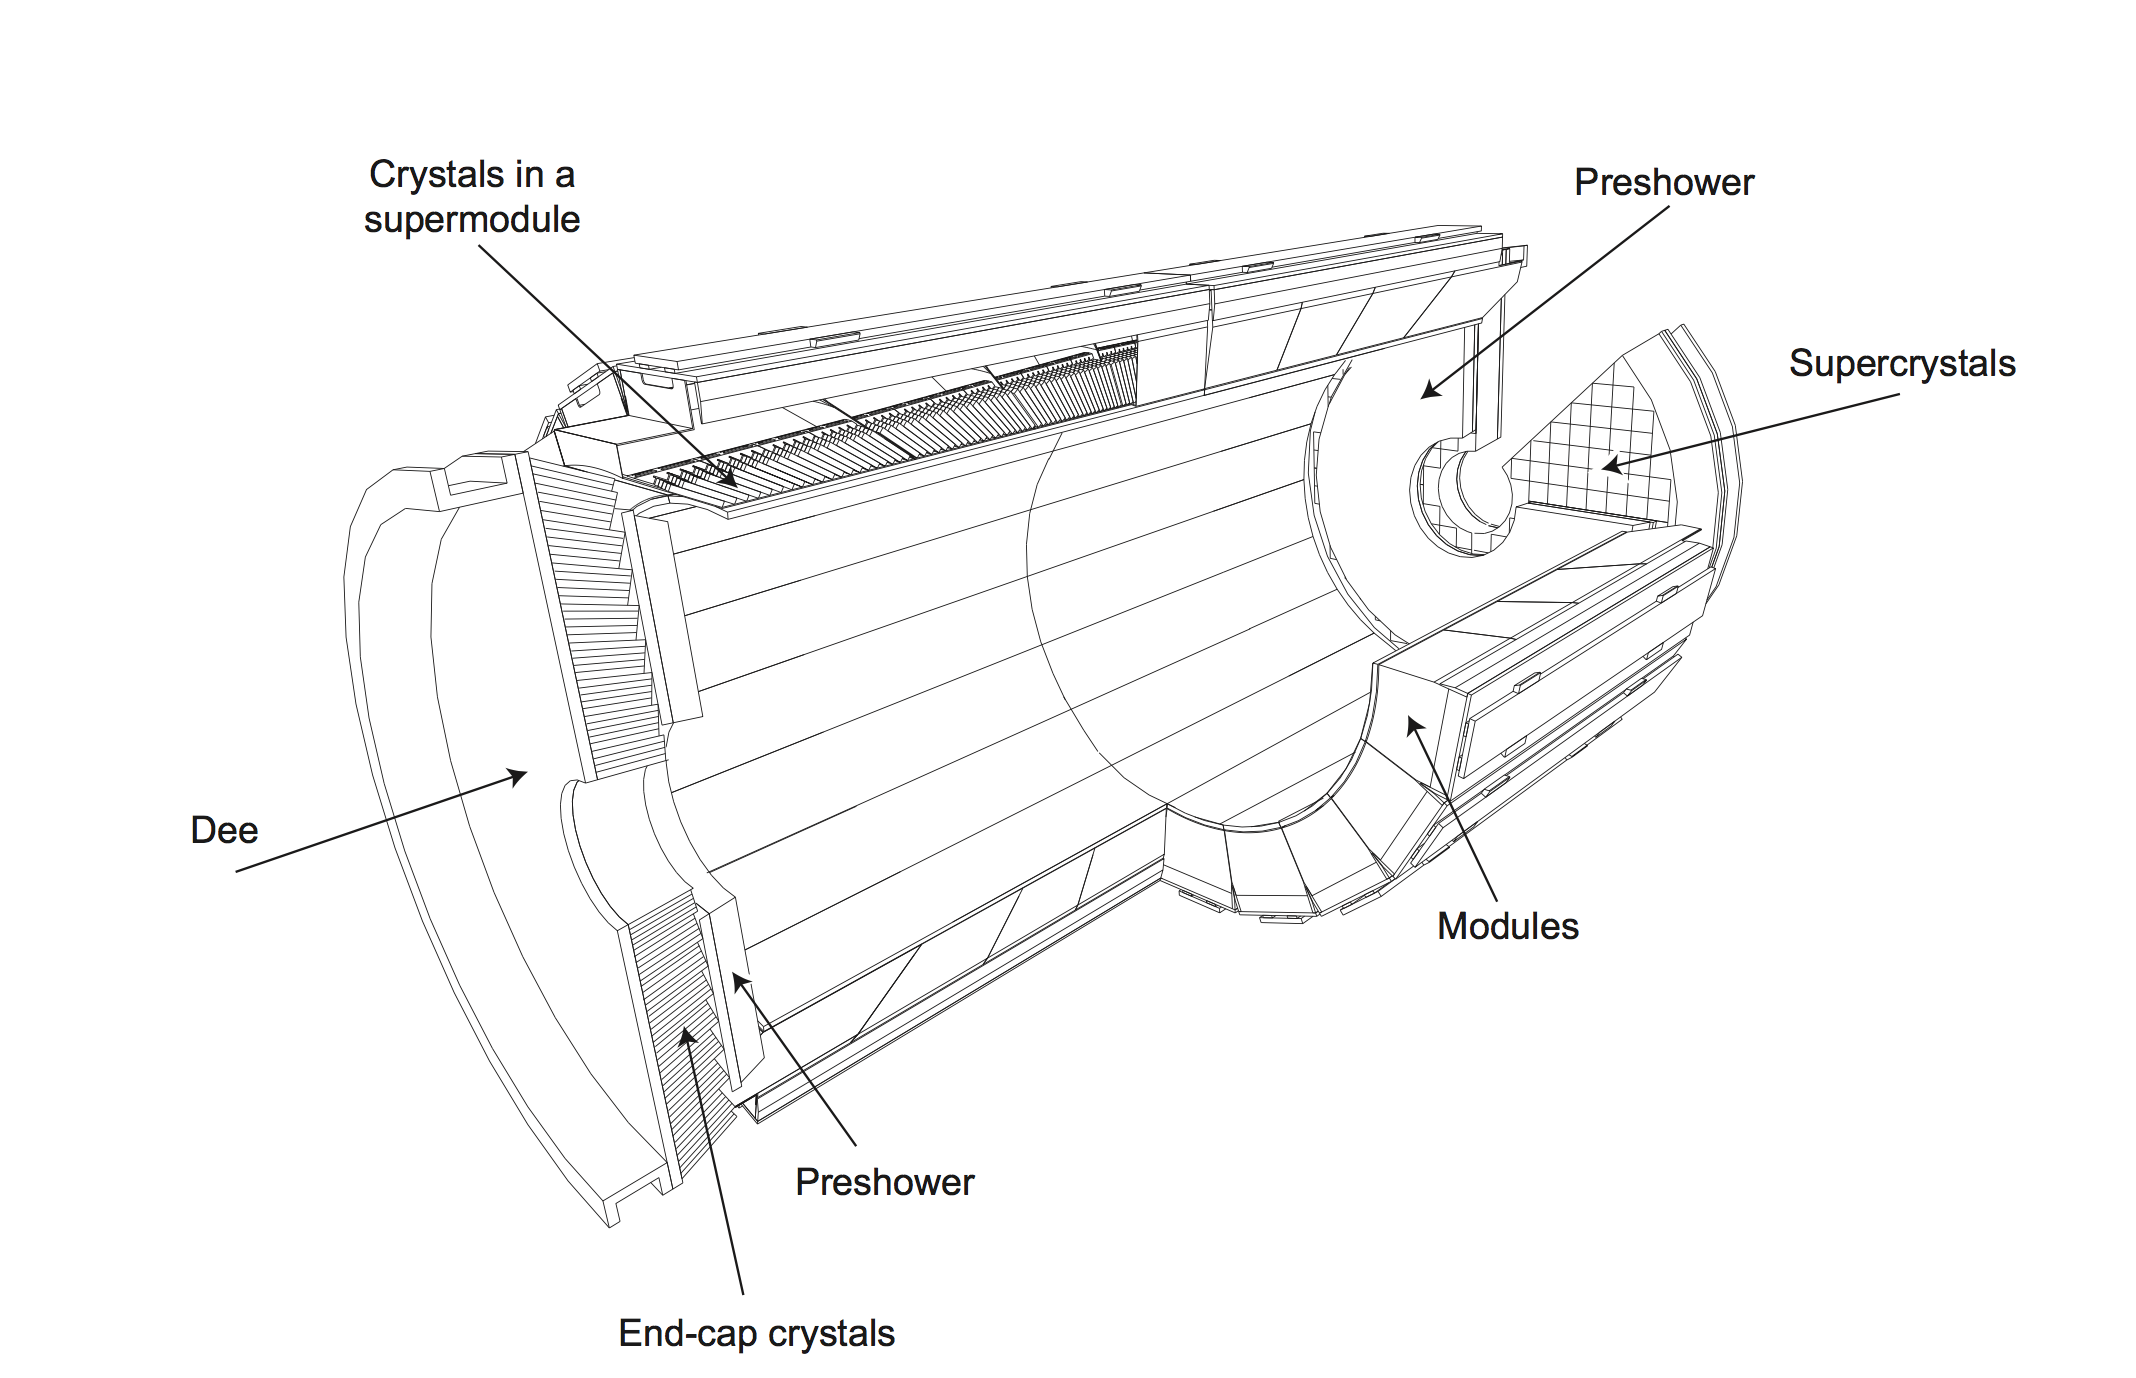
\includegraphics[width=0.9\textwidth]{./Detector/Plots/ECAL.png}
\caption[Layout of the ECAL, indicating the positions
of the different components.]{Layout of the \ac{ECAL}, indicating the position of the
different components \cite{cms-jinst}.}
\label{fig:CMS_ECAL}
\end{center}
\end{figure}

To preserve the energy resolution the crystals and
photodetectors need to be kept stable within $18\pm 0.05^{\circ}$C
as the number of scintillation photons emitted by the crystals,
and the amplification of the photodetectors, are temperature dependent.
This nominal operating temperature is ensured by 
supplying the detector with water at the same temperature.

The energy resolution of the \ac{ECAL} can be parameterised as
\begin{equation}\label{eqn:ecalres}
\frac{\sigma}{E} = \frac{S}{\sqrt{E}}\oplus\frac{N}{E}\oplus C,
\end{equation}
where $S$ is the stochastic term, $N$ the noise term and $C$ the constant term.
The stochastic term arises from fluctuations in lateral shower containment and 
fluctuations in the scintillation yield, the noise term is due to noise from the electronics
and additional particles in the event, and the constant term comes
from crystal-to-crystal intercalibration errors, the non-uniformity of the longitudinal response and 
energy leakage from the back of the crystals.

The values of $S$, $N$ and $C$ have been measured in an electron
test-beam, without a magnetic field or material in front of the \ac{ECAL}, as 
$S = 0.028\,\GeV^{\frac{1}{2}}$, $N = 0.12\,\GeV$ and $C= 0.003$.
%S = 2.83 %pm 0.03%, C = 0.26% pm 0.04%

\subsection{Hadron calorimeter}
\label{sec:CMSLHC_CMS_hcal}
The \ac{ECAL} is surrounded by the \ac{HCAL} \cite{cms-jinst}, which is needed for the
measurement of the energies of strongly interacting particles. As
the \ac{ECAL} extends out to a radius of $1.77\,\metre$ and the magnet coil
starts at a radius of $2.95\,\metre$, space for the \ac{HCAL} inside the magnet
coil is limited. The \ac{HCAL} design takes
this into account by placing part of the calorimeter outside the magnet coil. An
illustration of a quadrant of the
\ac{HCAL}, indicating the positions of the sub-systems, is shown
in figure \ref{fig:CMS_HCAL}.

\begin{figure}[h!]
\begin{center}
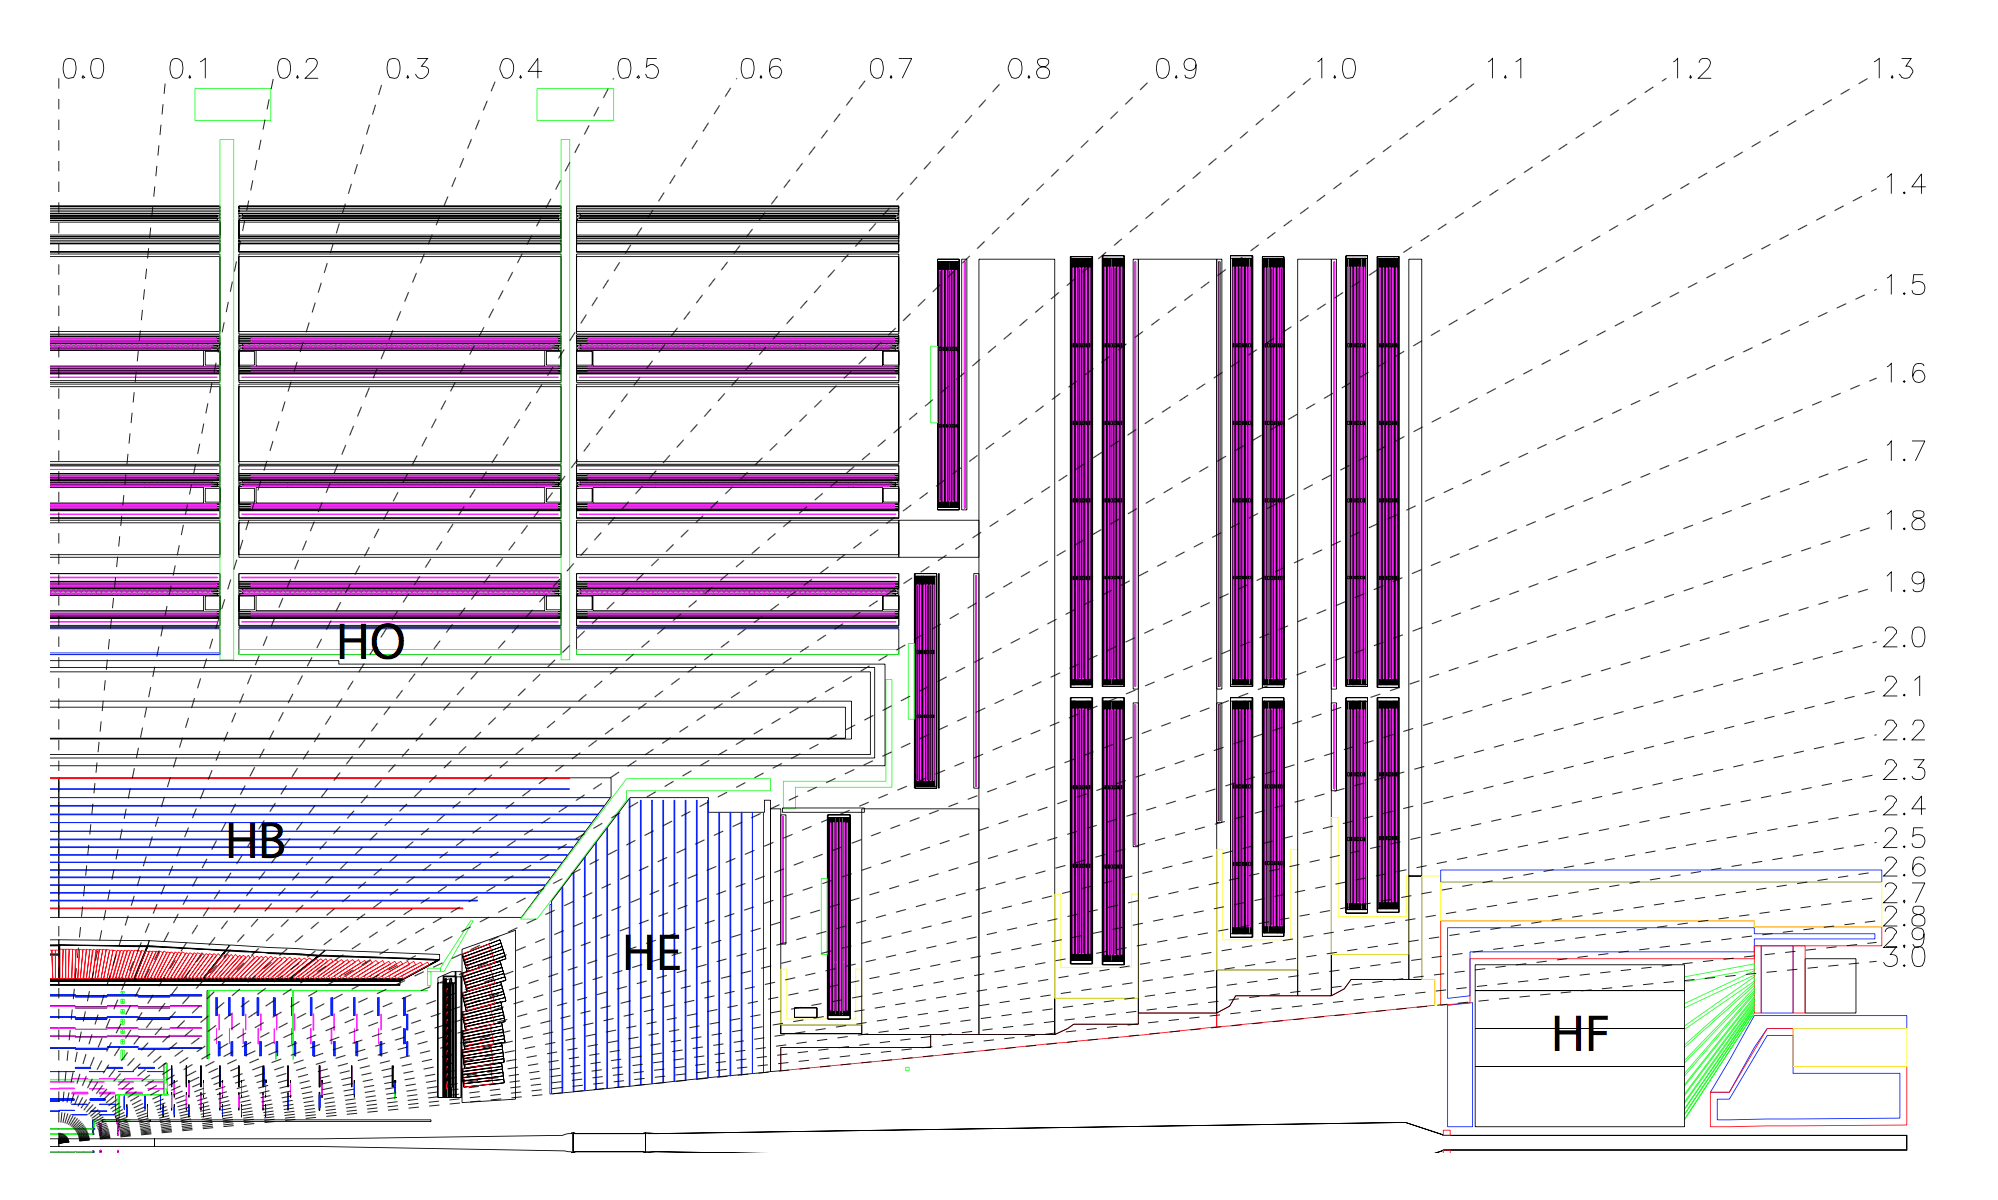
\includegraphics[width=0.9\textwidth]{./Detector/Plots/HCAL.png}
\caption[Illustration of a quadrant of the HCAL, showing the different
sub-systems of the detector.]{Illustration of a quadrant of the \ac{HCAL}, showing the different
sub-systems of the detector \cite{cms-jinst}.}
\label{fig:CMS_HCAL}
\end{center}
\end{figure}

In the barrel region the \ac{HB} provides
coverage up to $|\eta|<1.3$. Beyond this $\eta$ range the \ac{HE} covers
the region up to $|\eta|<3$. The \ac{HB} and \ac{HE} are sampling calorimeters made of brass absorber
plates with tiles of plastic scintillator as the active material. The brass used as 
absorber fits the constraints imposed by the environment due to its short interaction length
%Nuclear interaction length is the mean path length required to reduce the numbers of relativistic charged particles by the factor 1/e, or 0.368, as they pass through matter.
%Nuclear interaction length is the mean distance travelled by a hadronic particle before undergoing an inelastic nuclear interaction.
of $16.42\,\cm$ and the fact that it is non-magnetic. The tiles of scintillator 
are $0.087 \times 0.087$ in $\eta$-$\phi$ for $|\eta|<1.6$ and $0.17\times0.17$ in $\eta$-$\phi$
beyond this range. The light from each tile is collected with a wavelength-shifting fibre, 
which is read out using hybrid photodiodes. 

In the barrel the \ac{HCAL}
has a thickness of between 5.82 and 10.6 interaction lengths, which is not 
sufficient to identify, for example, late-starting showers. The \ac{HO}, sitting
outside of the magnet and using the coil as an additional absorber, extends the 
thickness to at least 11.8 interaction lengths. 
As in the \ac{HB} the active material of the \ac{HO} consists of plastic scintillator tiles which roughly
map the granularity of the tiles in the \ac{HB}, and are read out via the same mechanism. %by feeding the light
%to a hybrid photodiode via wavelength-shifting fibres.
%WTF: wavelength-shifting fibres

The \ac{HF}, providing coverage in the very forward region, is 
subjected to large radiation doses. This means an extremely radiation-hard
active material is needed. 
For this reason quartz
fibres are used. These fibres are embedded
in a steel absorber structure. Charged particles from the
shower initiated in the steel generate Cherenkov light in 
the quartz fibres, which is read out by photomultiplier tubes.
%Half of the fibres run over the full depth of the absorber
%while the other half starts at a depth of 22 cm, this is
%to distinguish electrons and photons (which deposit a large
%fraction of their energy in the first 22cm) from hadrons.

The energy resolution of the \ac{HCAL} for single charged pions 
was measured in a test beam \cite{cms-hcalecal}
and can be parameterised as 
\begin{equation}\label{eqn:hcal_res}
\frac{\sigma}{E} = \frac{S}{\sqrt{E}} \oplus C,
\end{equation}
where $S$ is the stochastic term, found to be 94.3\% %pm 1.2
and $C$ is the constant term, measured to be 8.4\%. %pm 1.0

%UPGRADE
During \ac{LS1} the photomultiplier tubes of the \ac{HF} were upgraded. The photomultiplier tubes and
read-out systems of other parts of the \ac{HCAL} will be upgraded in stages over the
next few years \cite{cms-hcal-upgrade}.

\subsection{Muon system}
\label{sec:CMSLHC_CMS_muons}
Accurate muon identification is one of the requirements of the \ac{CMS} 
experiment. High muon identification efficiency and precise muon momentum 
resolution are key to the success of the experiment, as muons are
very important for the detection of $\PHiggs\rightarrow \PZ\PZ \rightarrow 4\ell$ decays. In addition to that,
muons appear in the final states of many of the \ac{BSM} signatures the experiment is searching for.

The \ac{CMS} muon system \cite{cms-jinst} is composed of three sub-systems which
are all necessary to ensure the identification requirements can be met. The muon system is located
outside of the magnet coil, interspersed in the iron return yoke of the solenoid.
In the barrel of the detector the \acp{DT} provide coverage for $|\eta|<1.2$, with
the \acp{CSC} covering the $0.9<|\eta|<2.4$ region. The \acp{RPC}, covering the same
regions as both the \acp{DT} and \acp{CSC}, are used as a dedicated triggering system.

A cross section of one quadrant of the detector, indicating
the positions of the \acp{DT}, \acp{CSC} and \acp{RPC}, is shown in figure \ref{fig:CMS_MuonSystem}.
The top of the fourth muon endcap station as shown in this figure was added during \ac{LS1} \cite{cms-muon-upgrade}, providing
additional layers of \acp{CSC} and \acp{RPC}.
\begin{figure}[h!]
\begin{center}
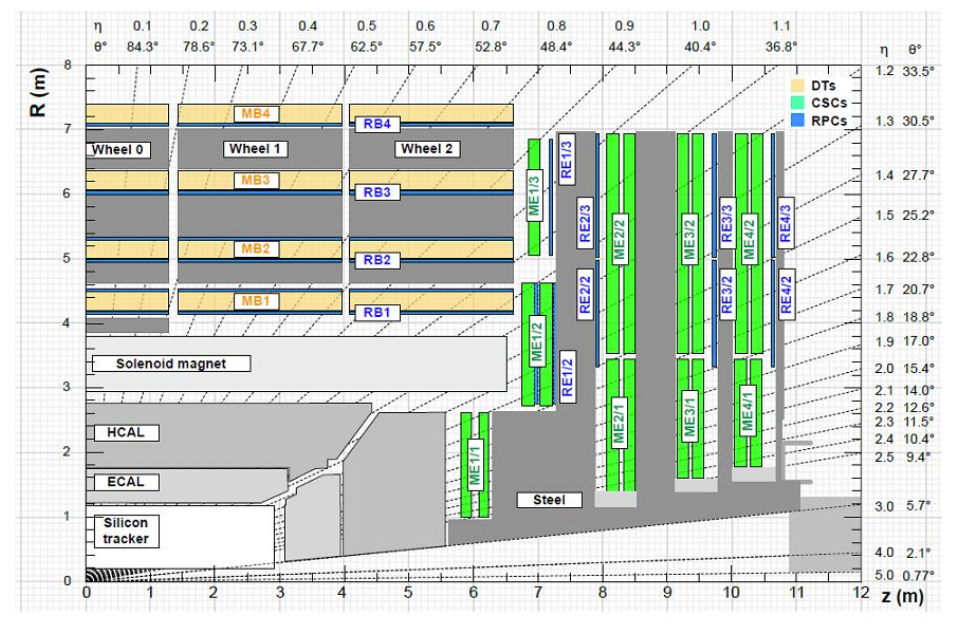
\includegraphics[width=0.8\textwidth]{./Detector/Plots/MuonSystemUpgrade.png}
\caption[Cross section of one quadrant of the CMS detector,
indicating the positions of the different muon system components.]{Cross section of one quadrant of the CMS detector, indicating
the positions of the different muon system components \cite{cms-muon-upgrade}. The 
fourth muon endcap stations were extended during \ac{LS1}; in Run 1 only the lower
part existed.}
\label{fig:CMS_MuonSystem}
\end{center}
\end{figure}

The \acp{DT} consist of layers of drift cells which have a cross section of $4.2\,\cm \times 1.3\,\cm$ and
are $2.4\,\metre$ long. The cells are filled with a mixture of %85\% 
argon gas and carbon dioxide gas.
Muons passing through the chamber ionise the gas, freeing electrons
which drift towards the anode wire running along the centre of the tube-shaped cell. 
This gives rise to an electric signal. There are four drift tube stations in each wedge of 
the detector, each in turn consisting of 8 to 12 layers of drift tubes. Some of
these layers are oriented parallel to the beam line, providing a measurement of $\phi$.
There are also layers oriented orthogonal to the beam line, which give a measurement
of the $z$ coordinate. Measurements of the spatial resolution were made
during p-p running in 2010.
The spatial resolution of the \acp{DT} is $80$--$120\,\micron$ per chamber for
measurements in the $\phi$ direction, while the resolution of the $z$ measurement
is $130$--$400\,\micron$ \cite{cms-muon-7tev}. %Drift lines distorted by magnetic field parallel to the wires

In the endcaps, where both the muon rate and the radiation levels are higher, the \acp{CSC} provide
measurements of the muon track. These detectors are radiation hard,
and have a fast response and fine segmentation.
Each of the \ac{CSC} modules is a wedge-shaped
multi-wire proportional chamber %WTF
with six gaseous chambers bounded by cathode plates. Sensitive
strips are placed on these plates in the 
radial direction, to measure the muon coordinate in the  $r$--$\phi$ plane.
Anode wires between the cathode planes
run along the \mbox{$\phi$ direction} and provide a measurement of
$\eta$. The resolution of the $r$--$\phi$ measurement is $40$--$120\,\micron$ \cite{cms-muon-7tev}.

In addition to the \acp{DT} and \acp{CSC}, the \acp{RPC} provide coverage
for $|\eta|<1.6$. These are made up of parallel plates, forming the anode and cathode,
with a gas gap in between. Ionisation of the gas due to the passing
muons is read out using aluminium strips running parallel to the 
beam axis. The position resolution of the \acp{RPC} is poorer than
that of the \acp{DT} and \acp{CSC}, but their time response is very fast. As
a result of this the \acp{RPC} are used as an independent muon trigger
which can correctly identify the beam crossing from which the muon
originated.

To obtain precise muon momentum resolution, information from 
the tracker hits has to be combined with measurements in the
muon stations. The momentum resolution of the muon system
alone is 9\% for muons with \pT~up to $200\,\GeV$, and varies with $\eta$ 
between $15$--$40\%$ for muons with \pT~of $1\,\TeV$ \cite{cms-jinst}. %ADD FORMULA

%Because of the uncertainty in the eventual background rates and in the ability of the muon system to measure the correct beam-crossing time when the LHC reaches full luminosity, a com- plementary, dedicated trigger system consisting of resistive plate chambers (RPC) was added in both the barrel and endcap regions. The RPCs provide a fast, independent, and highly-segmented trigger with a sharp pT threshold over a large portion of the rapidity range (|η| < 1.6) of the muon system. The RPCs are double-gap chambers, operated in avalanche mode to ensure good operation at high rates. They produce a fast response, with good time resolution but coarser position reso- lution than the DTs or CSCs. They also help to resolve ambiguities in attempting to make tracks from multiple hits in a chamber.

\subsection{Triggering and data processing}
\label{sec:CMSLHC_CMS_trigger}
When the \ac{LHC} is operating under design conditions, protons are collided at a rate
of $40\,$MHz. This rate is too high for the \ac{DAQ} system to read out every event. In
addition this high collision rate produces such a large number of events that it would
not be feasible to write every single event, with a size of around 1 MB, to tape. Therefore, a trigger
system is used to select events of interest, which reduces the rate
at which events are stored to  $\mathcal{O}(1 \text{ kHz})$.

The trigger system consists of two stages: the \ac{L1} trigger and the \ac{HLT}. 
The \ac{L1} trigger only makes use of front-end electronics and reduces the event rate 
from $40\,$MHz to around $100\,$kHz. The \ac{HLT} 
runs on a computer farm with around $13\,000$ CPU cores \cite{cms-trigger}.
During \ac{LS1} and the year-end technical stop at the end of 2015 the \ac{L1} trigger was
replaced by a completely upgraded system \cite{cms-trigger-tdr}, which provides, amongst other 
things, improved object isolation, hadronic tau identification, muon \pT~resolution and
jet finding with respect to the system used during Run 1.
An overview of the data flow in the \ac{L1} trigger is given in figure \ref{fig:CMS_Trigger}.

\begin{figure}[h!]
\begin{center}
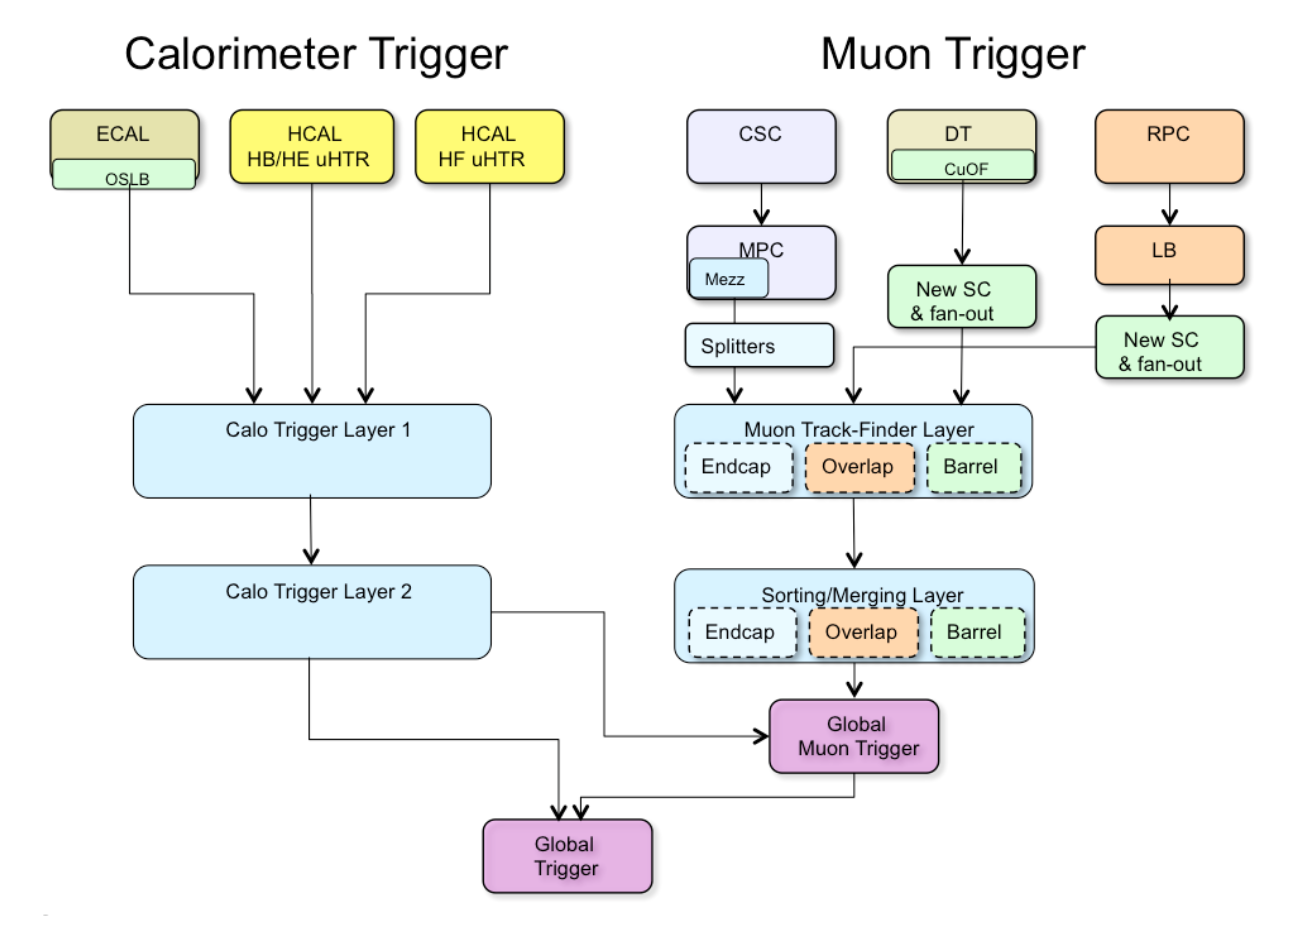
\includegraphics[width=\textwidth]{./Detector/Plots/CMSTrigger.png}
\caption[Schematic of the different components of the L1 trigger.]{Schematic of the different components of the \ac{L1} trigger \cite{cms-trigger-tdr}.}
\label{fig:CMS_Trigger}
\end{center}
\end{figure}

The \ac{L1} trigger only makes use of information from the calorimeters and the muon systems.
The calorimeter trigger starts from \ac{HCAL} and \ac{ECAL} energy deposits, 
which are fed to the first layer of the trigger, where it makes use of a time-multiplexed system. 
The first trigger layer maps onto slices of the detector, receiving data from many bunch crossings. These data are passed
on to the second layer of the trigger in a way that bundles data from a single bunch crossing, but
different slices of the detector, to be processed on one node in the second layer of the
trigger. In this step basic object identification is performed based on the energy
deposits, so that a sorted list of the best candidates can be passed to the global trigger.
The trigger employed during Run 1, and the first year of Run 2, did not use time-multiplexing. Instead, 
information from different regions of the detector was processed independently.

Hits in the muon chambers are read out and passed to the track finder layer 
of the muon trigger, which combines information from the \ac{CSC}, \ac{DT}
and \ac{RPC} systems in regions of $\eta$-$\phi$.
In further layers of the muon trigger the information from different
regions is combined, until finally the global muon trigger
can return a sorted list of the best muon candidates to the global trigger.
The global trigger combines the information from the calorimeter and muon triggers
to make a decision on whether the event should be sent to the \ac{HLT} or whether
it should be discarded. A decision has to be made within $3.2\,\micro\second$, the maximum time during
which data can be stored in the \ac{L1} trigger before being lost.

%The muon trigger is a tracking trigger that measures the momentum of muons using the magnetic field in the steel yoke of the CMS solenoid; thus its resolution degrades with increasing momentum. This can be improved by maximizing the number of chamber hits along a muon trajectory and by improving the precision and number of position and angular measurements participating in the track fit applied in the trigger logic. Moreover, isolation criteria can be applied using the energy deposits in the calorimeter in order to further reduce the rate of muons from heavy flavor jets.

The \ac{HLT}, running on CPU nodes, makes use of the full information
from the detector, including tracker hits. This means particles
can be more accurately identified and their momentum is more
precisely known. The algorithms used in the \ac{HLT} are usually simpler
versions of those used in the full offline reconstruction. %Can't use full because time limited
During the 2012 run of the \ac{LHC} the \ac{HLT} operated with an output
capacity of around $1\,$kHz. For Run 2 this has been increased. In August 2016 
the \ac{HLT} output rate was $1.2\,$kHz for immediate data processing, with
an additional $0.6\,$kHz saved as raw data to be reconstructed and analysed when 
more processing power is available \cite{CMS-PAS-HIG-16-037}. %ie at the end of run 2

While the trigger system reduces the rate substantially, several
petabytes of collision data are stored by \ac{CMS} each year, on top
of large sets of simulated events. 
To make these large amounts of data easily accessible for analysis, 
\ac{CMS} and the other \ac{LHC} experiments make use of the \ac{WLCG} \cite{lhc-wlcg}. 
The \ac{WLCG} pools the resources of computer centres at universities and research
laboratories associated with \ac{LHC} experiments, based on a system of tiers. The Tier 0, at \ac{CERN} and
the Wigner Research Centre for Physics in Budapest, performs the full reconstruction
and saves a copy of the data to tape. Datasets are copied to at least one Tier 1 centre, from
where data can be distributed to Tier 2 centres. The Tier 2 centres are located
at over 150 universities and research institutes around the world, providing 
resources for analysis of the datasets to all researchers associated with the experiment.



